\newpage
%%%%%%%%%%%%%%%%%%%%%%%%%%%%%%%%%%%%%%%%%%%%%%%%
%%%%%%%%%%%%%%%%%%%%%%%%%%%%%%%%%%%%%%%%%%%%%%%%
\section{Statistical Procedure}
To build a statistical model for this analysis we consider following sources of systematics
shared (100\% correlated between channels):
\begin{itemize}
\item uncertainties in luminosity, jet energy scale, trigger efficiency
\item uncertainty of backgrounds: WZ, ZZ, Z$\gamma$, $t\bar{t}$, rare processes
\item uncertainty of electron reconstruction, identification, selection efficiencies
\item uncertainty of muon reconstruction, identification, selection efficiencies
\item uncertainty of tau reconstruction, identification, selection efficiencies
\end{itemize}
Every channel also has two nuisances uncorrelated with other channels.
These uncertainties account for statistical fluctuations affecting
background estimations, and signal efficiency calculation.
As the total number of nuisances is proportional to number of channels used,
and therefore necessary computing resources rise exponentially with number
of combined channels,
we have to keep number of channels actually used for the analysis limited.
For the given point in the model parameter space we select a predefined
number (currently 10) of the most sensitive
channels. The sensitivity of the channel is defined as an expected limit
on the total model cross section obtained by using this channel only.
This analysis is a typical multi-channel counting experiment. Higgs group combination
tool, LandS~\cite{lands}, is technically used to obtain limits.
We calculate ``LHC style'' CLs limit~\cite{higgsCombination},
which effectively means using frequentist CLs with one-sided profiled likelihood
test statistics.


%%%%%%%%%%%%%%%%%%%%%%%%%%%%%%%%%%%%%%%%%%%%%%%%
%%%%%%%%%%%%%%%%%%%%%%%%%%%%%%%%%%%%%%%%%%%%%%%%
\subsection{Limits on SMS from the search with three leptons and from same-sign di-lepton searches}
\label{tri-ss-combine}

Figure~\ref{fig:ULtriA} displays, for $\xslep = 0.5$, 
the results of the three-lepton search using $\MET$, $\MT$ and $\mdil$. 
The figure depicts 95\% CL upper limit on the cross section times branching fraction in the $m_{\chiz_1}$
versus $m_{\chiz_2}$ ($=m_{\chipm_1}$) plane in the flavor-democratic scenario.
%described in the Introduction.  
The contour bounds the excluded region in the plane assuming the NLO cross section
calculation and a 50\% branching fraction, as appropriate for the visible decay products in this scenario.
Figure~\ref{fig:ULtriAss} shows the results for two values $\xslep$ (0.05 and 0.95)
obtained after combination of three-lepton and the SS di-lepton searches~\cite{AN-2012:330}.
%==========================================================================================
\begin{figure}[!p]
\begin{center}
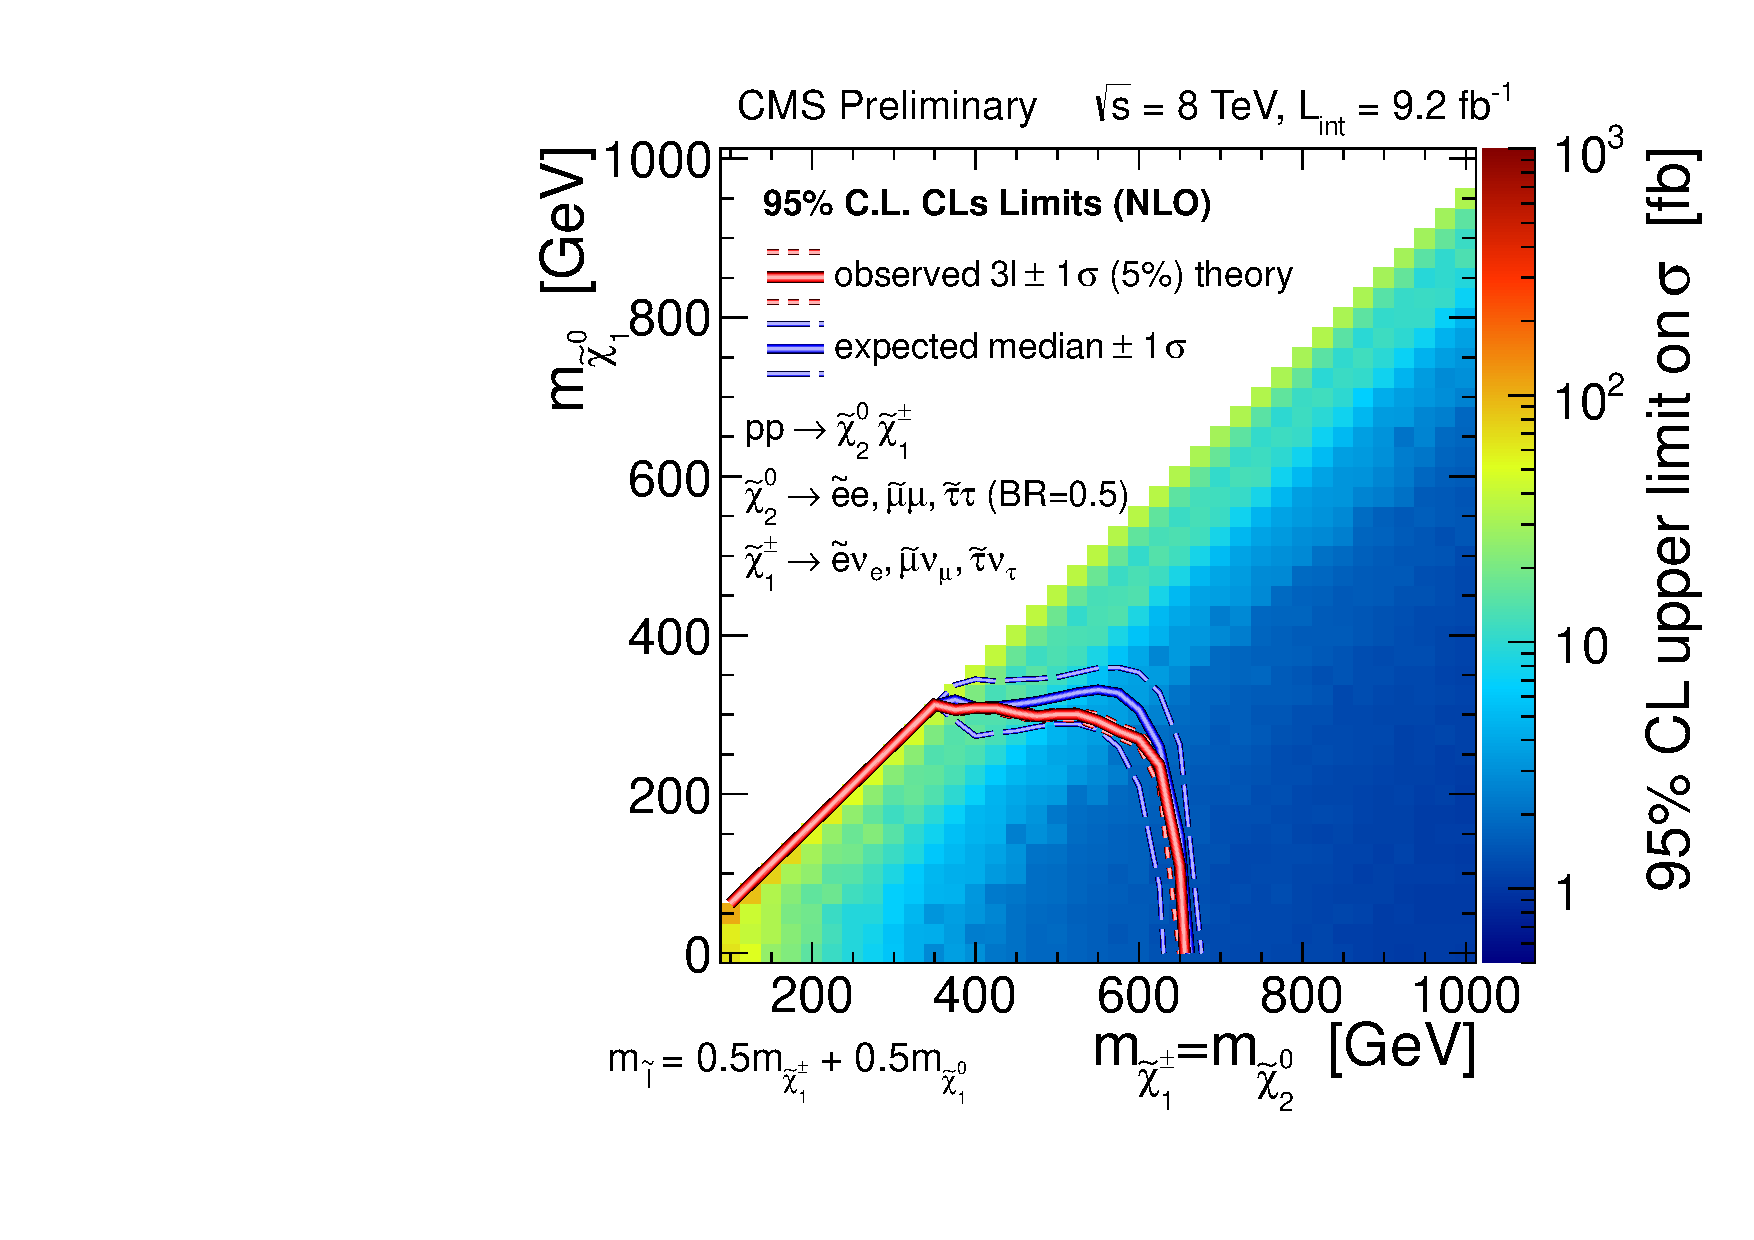
\includegraphics[width=0.8\textwidth]{plots/exclusions/exclusion_TChiSlepSnu_2i_0_5.pdf} 
\caption{
The shading in the $m_{\chiz_1}$ versus $m_{\chiz_2}$
($=m_{\chipm_1}$) plane indicates the 95\% CL upper limit on the
chargino-neutralino production NLO cross section times branching fraction
in the flavor-democratic scenario, for the 
three-lepton search.  The contours bound the mass regions excluded at 95\%
CL for a branching fraction of 50\%, as appropriate for the visible
decay products in this scenario. The contours based on the
observations are shown; in addition, the expected bound is shown. }
\label{fig:ULtriA}
\end{center}
\end{figure}
%==========================================================================================
%==========================================================================================
\begin{figure}[!p]
\begin{center}
\subfigure[$\xslep = 0.05$]{\label{fig:ULtriAss1}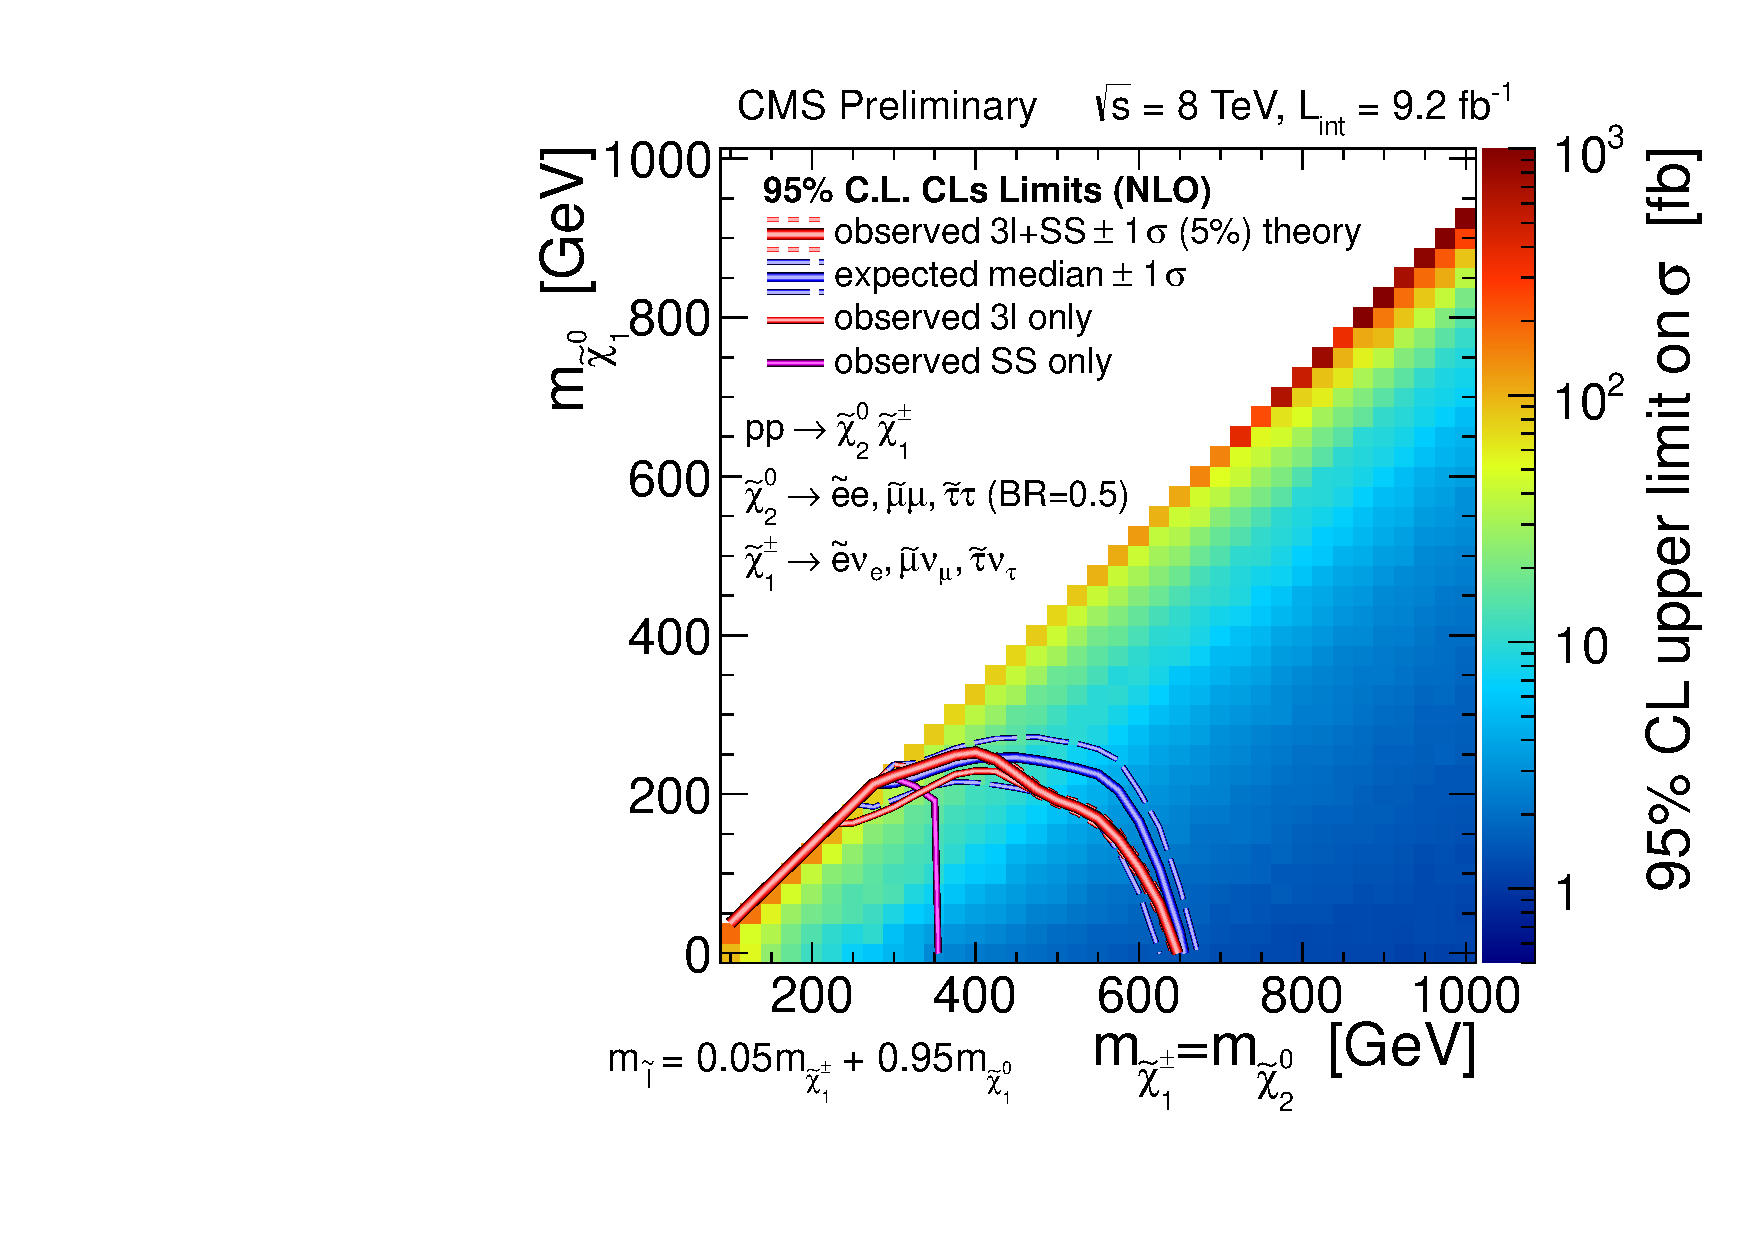
\includegraphics[width=0.5\textwidth]{plots/exclusions/exclusion_TChiSlepSnu_2i_0_05.pdf} }
\subfigure[$\xslep = 0.95$]{\label{fig:ULtriAss3}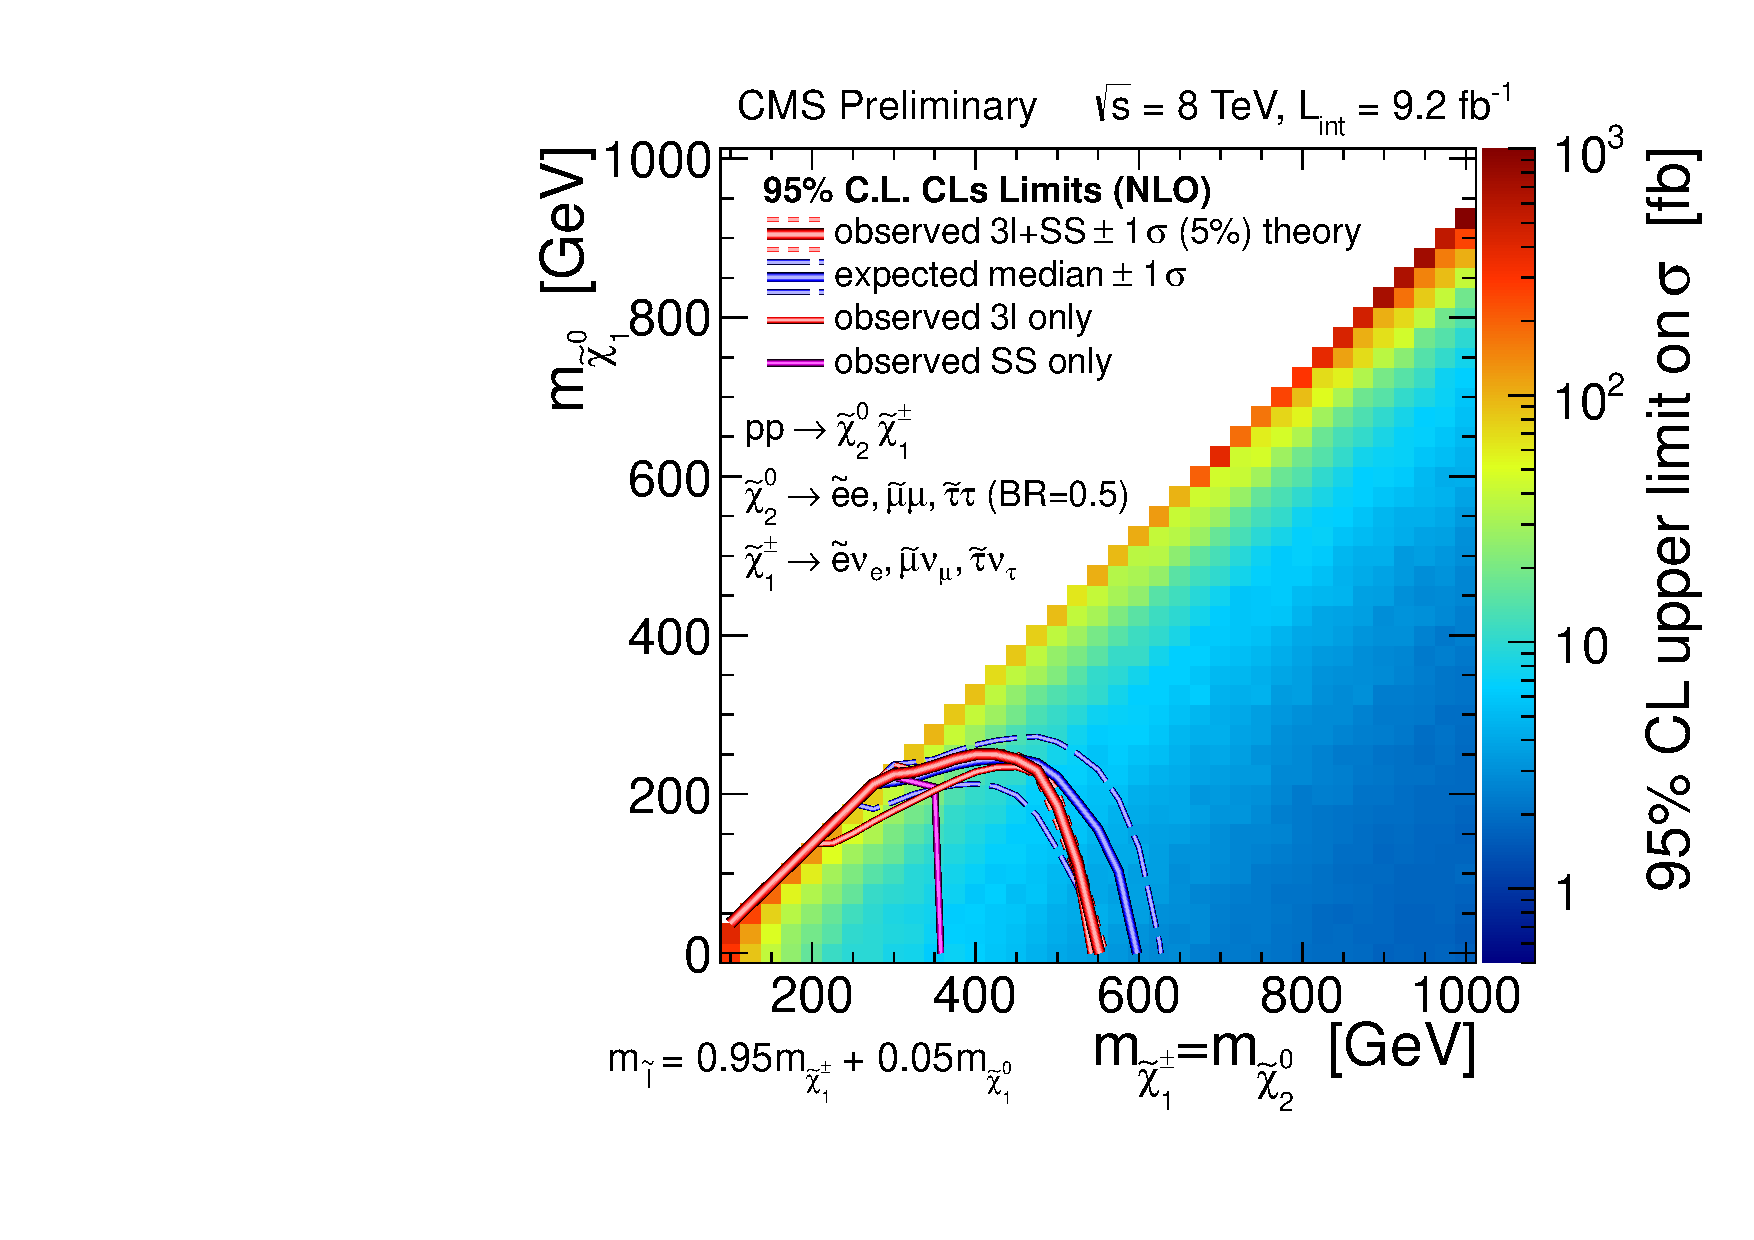
\includegraphics[width=0.5\textwidth]{plots/exclusions/exclusion_TChiSlepSnu_2i_0_95.pdf} }
\caption{
The shading in the $m_{\chiz_1}$ versus $m_{\chiz_2}$
($=m_{\chipm_1}$) plane indicates the 95\% CL upper limit on the
chargino-neutralino production NLO cross section times branching fraction
in the flavor-democratic scenario, for the combined analysis of the
three-lepton search and the same-sign di-lepton search.  
The contours bound the mass regions excluded at 95\%
CL for a branching fraction of 50\%, as appropriate for the visible
decay products in this scenario. The contours based on the
observations are shown for the combination; in addition, the expected 
combined bound is shown. Red contours demonstrate separate mass exclusions 
for the three-lepton search and the same-sign di-lepton search alone.
}
\label{fig:ULtriAss}
\end{center}
\end{figure}
%==========================================================================================

Figure~\ref{fig:ULtriB} presents the corresponding limits for the $\tau$-enriched scenario 
and Figure~\ref{fig:ULtriC} for the $\tau$-dominated scenario.  
As the SS di-lepton search does not have sensitivity for $\xslep=0.50$, there is no limit curve for this search
for Figures~\ref{fig:ULtriA},~\ref{fig:ULtriB2} and~\ref{fig:ULtriC}.  In the other limit curves in both
Figures~\ref{fig:ULtriAss} and~\ref{fig:ULtriB}, the increase in the
combined mass limit from incorporation of the SS di-lepton search
ranges up to approximately $20\GeV$.

%==========================================================================================
\begin{figure}[!p]
\begin{center}
\subfigure[$\xslep = 0.05$]{\label{fig:ULtriB1}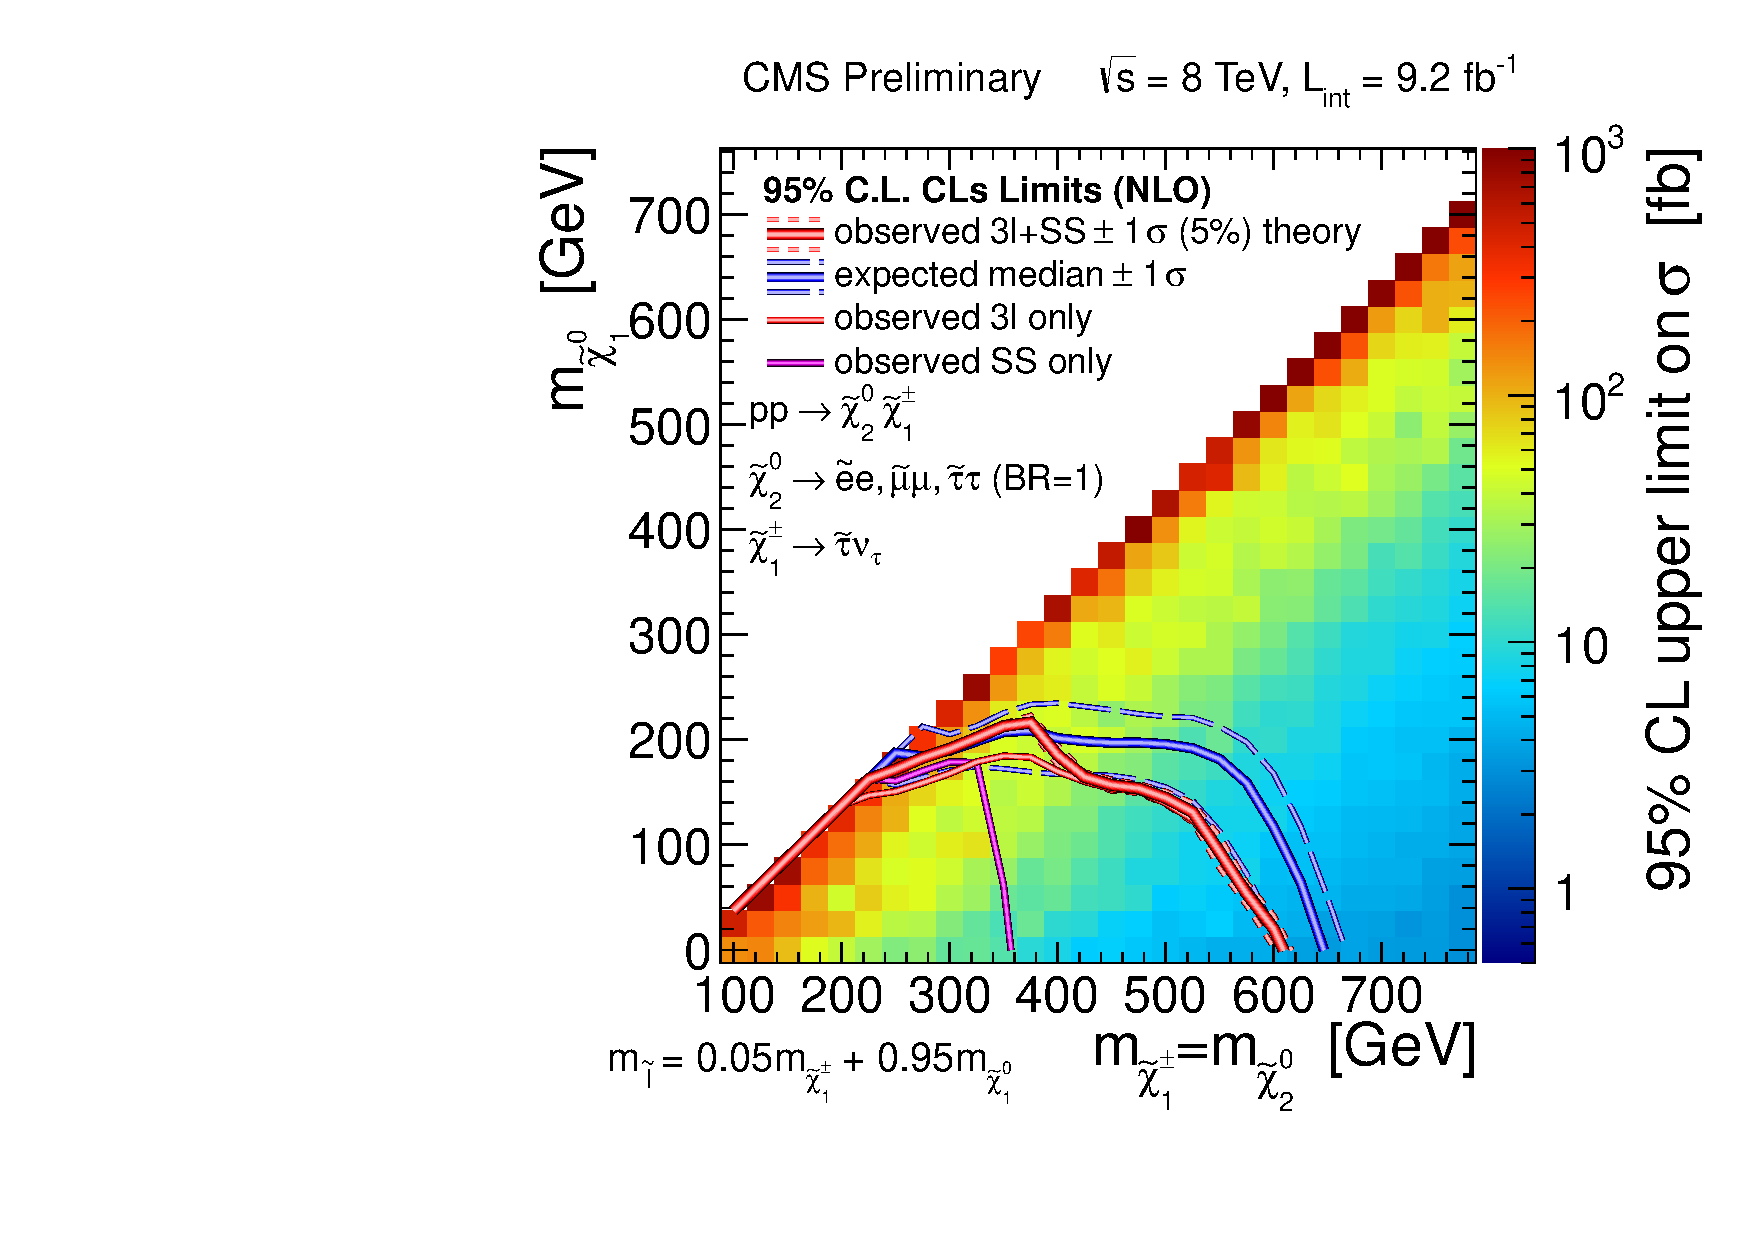
\includegraphics[width=0.5\textwidth]{plots/exclusions/exclusion_TChiSlepSnu_2a_0_05.pdf} }
\subfigure[$\xslep = 0.5$]{\label{fig:ULtriB2}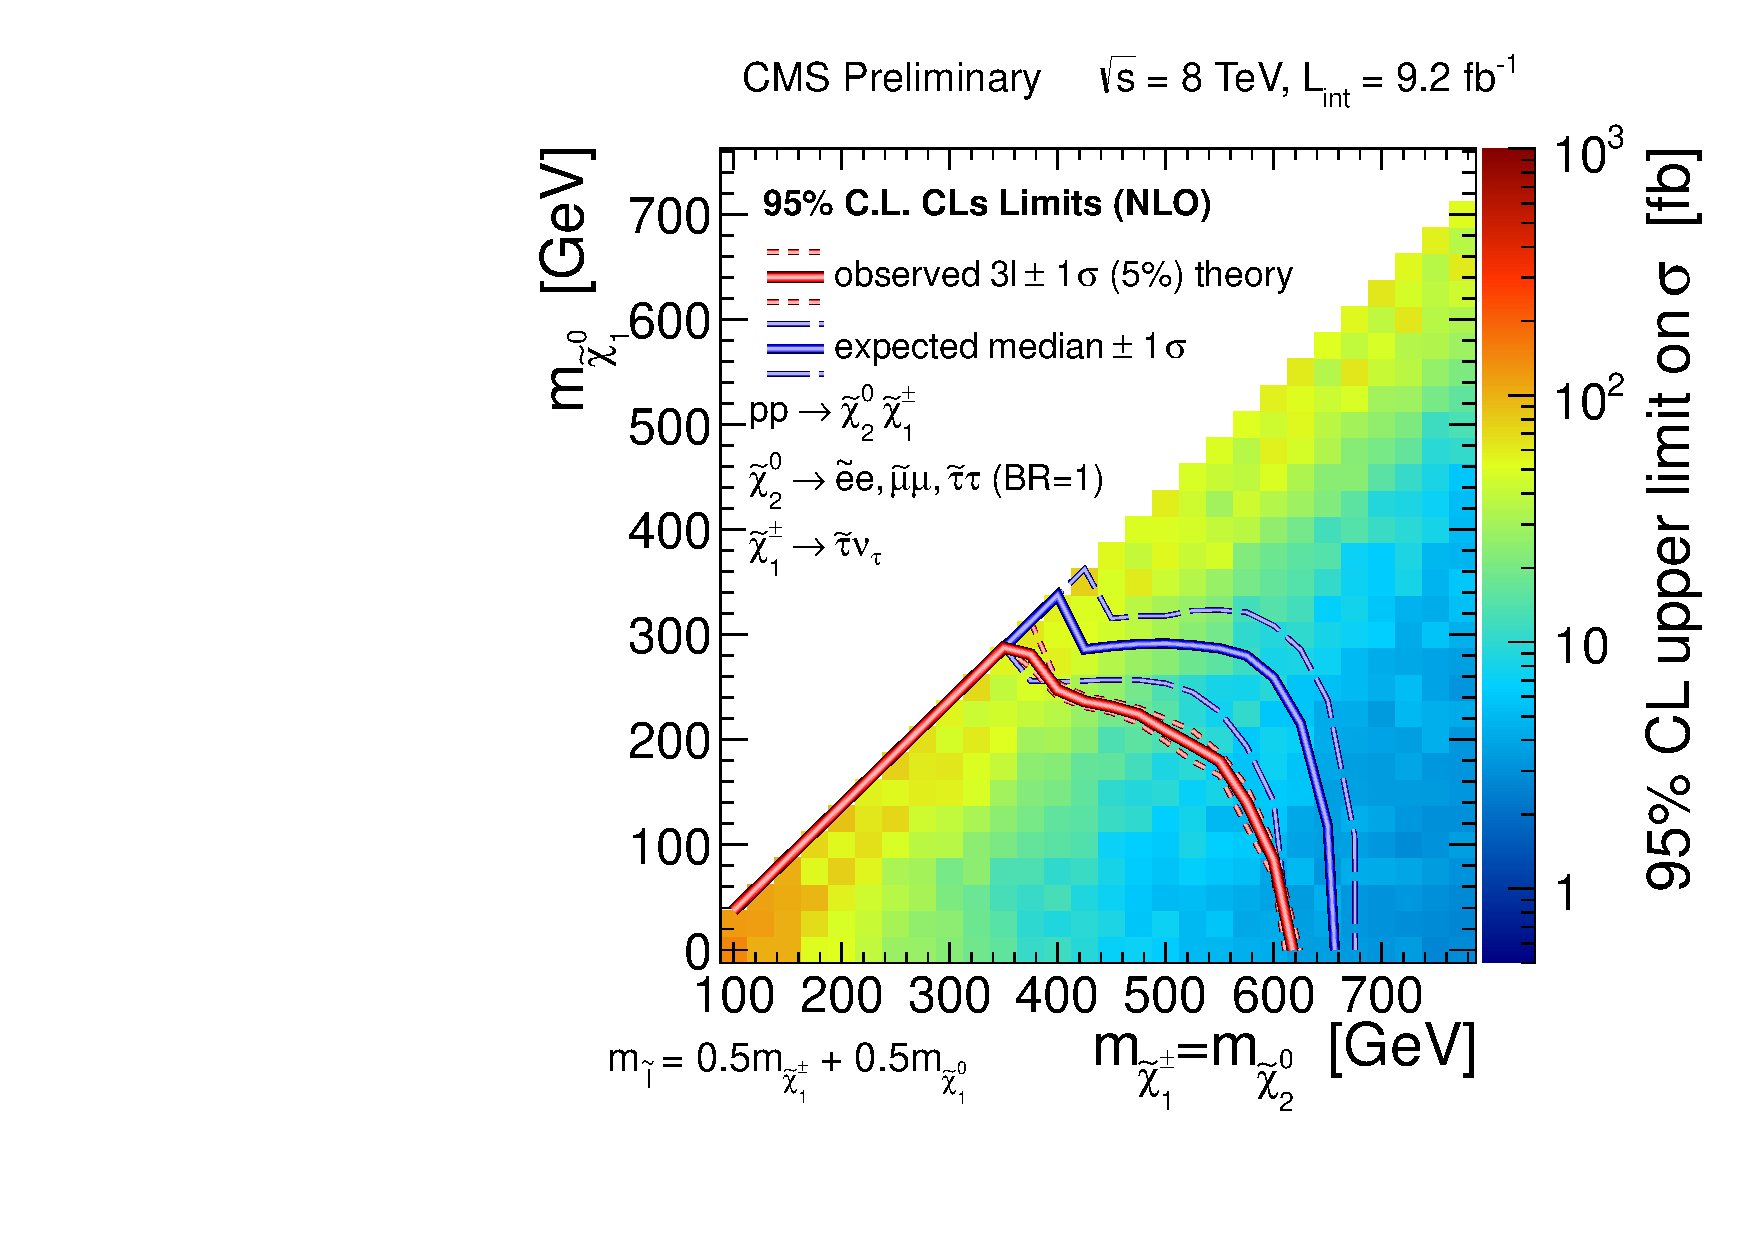
\includegraphics[width=0.5\textwidth]{plots/exclusions/exclusion_TChiSlepSnu_2a_0_5.pdf} } \\
\subfigure[$\xslep = 0.95$]{\label{fig:ULtriB3}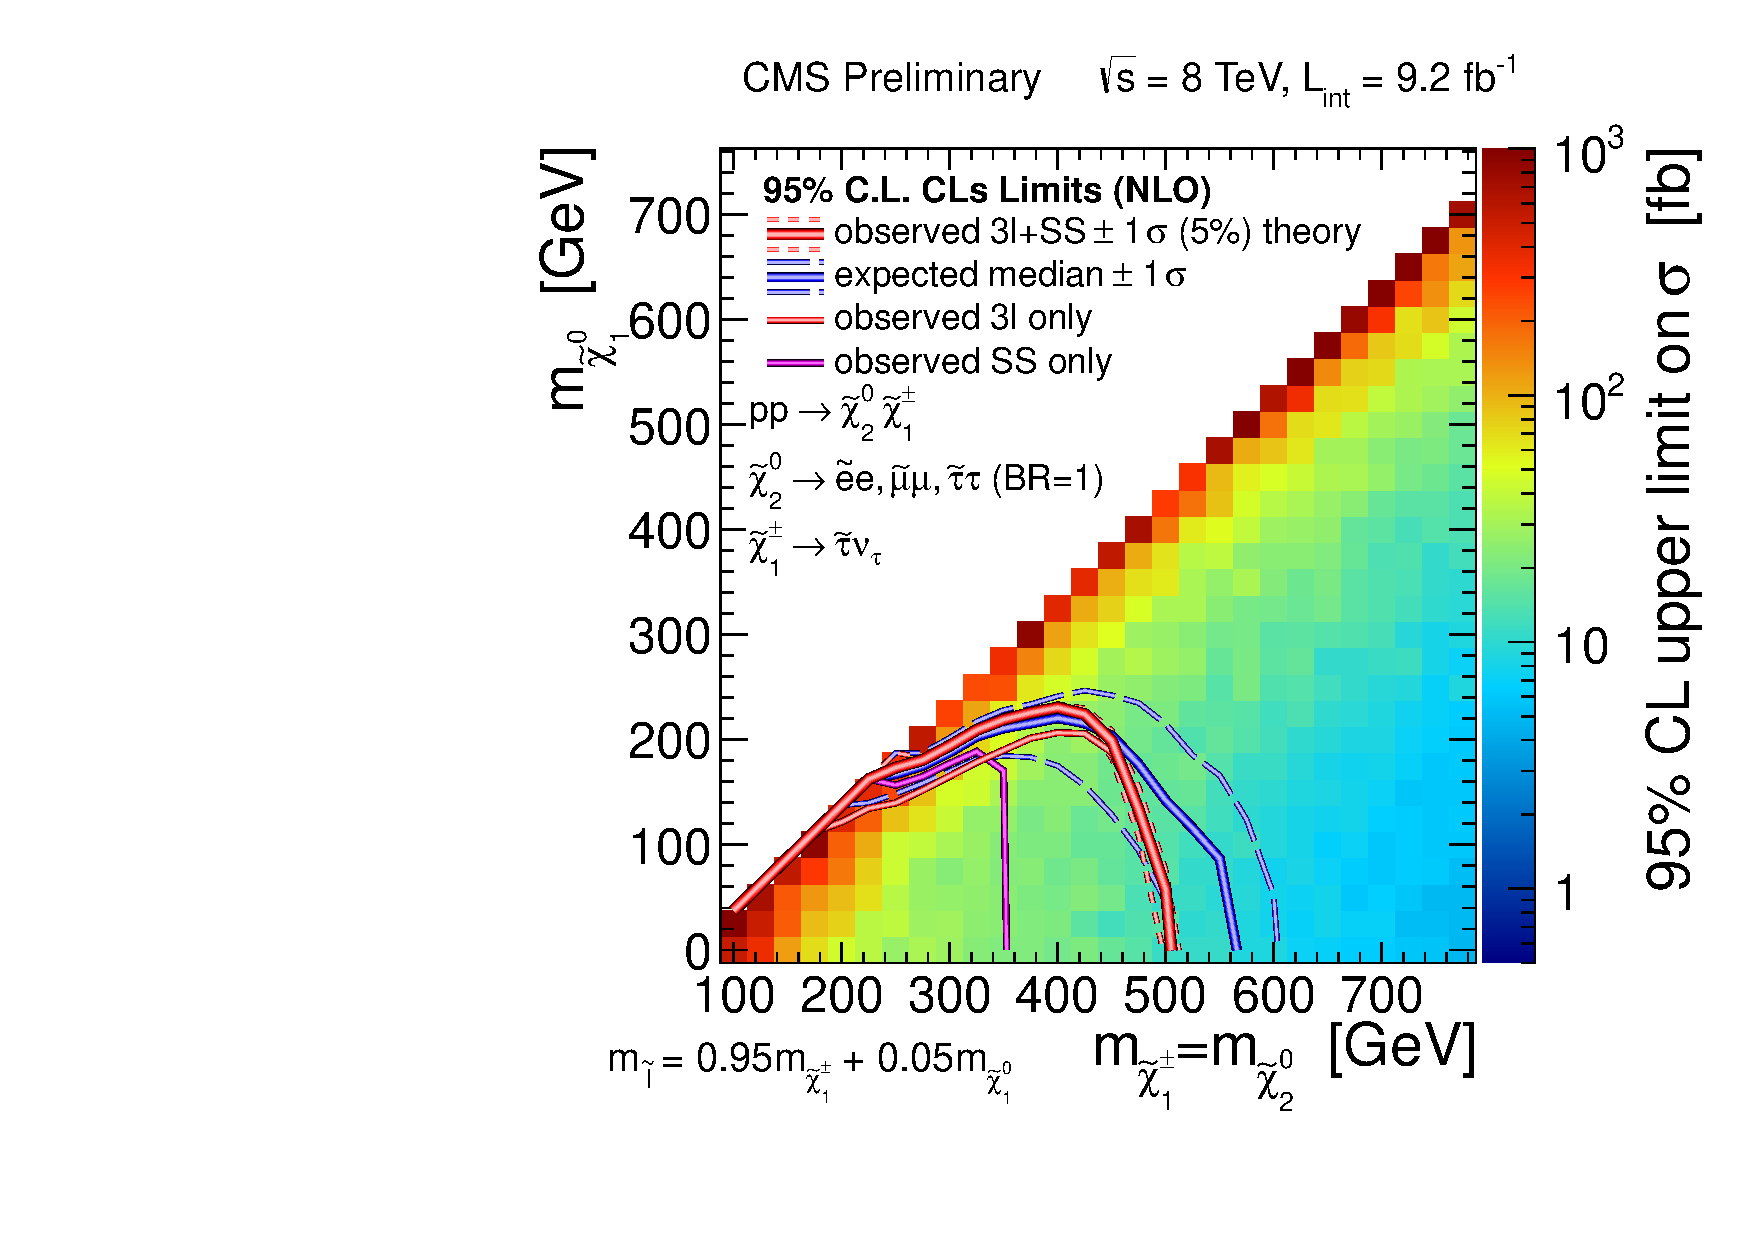
\includegraphics[width=0.5\textwidth]{plots/exclusions/exclusion_TChiSlepSnu_2a_0_95.pdf} }
\caption{The exclusion contours for $\tau$-enriched scenario corresponding to results in Figure~\ref{fig:ULtriA}: 
(a) and (c) combination of 3-lepton searches with SS d-lepton analysis, 
(b) 3 lepton searches.}
\label{fig:ULtriB}
\end{center}
\end{figure}
%==========================================================================================
%==========================================================================================
\begin{figure}[!p]
\begin{center}
%\subfigure[$\xslep = 0.05$]{\label{fig:ULtriC1}\includegraphics[width=0.33\textwidth]{plots/exclusions/xxx.pdf} }
\subfigure[$\xslep = 0.5$]{\label{fig:ULtriC2}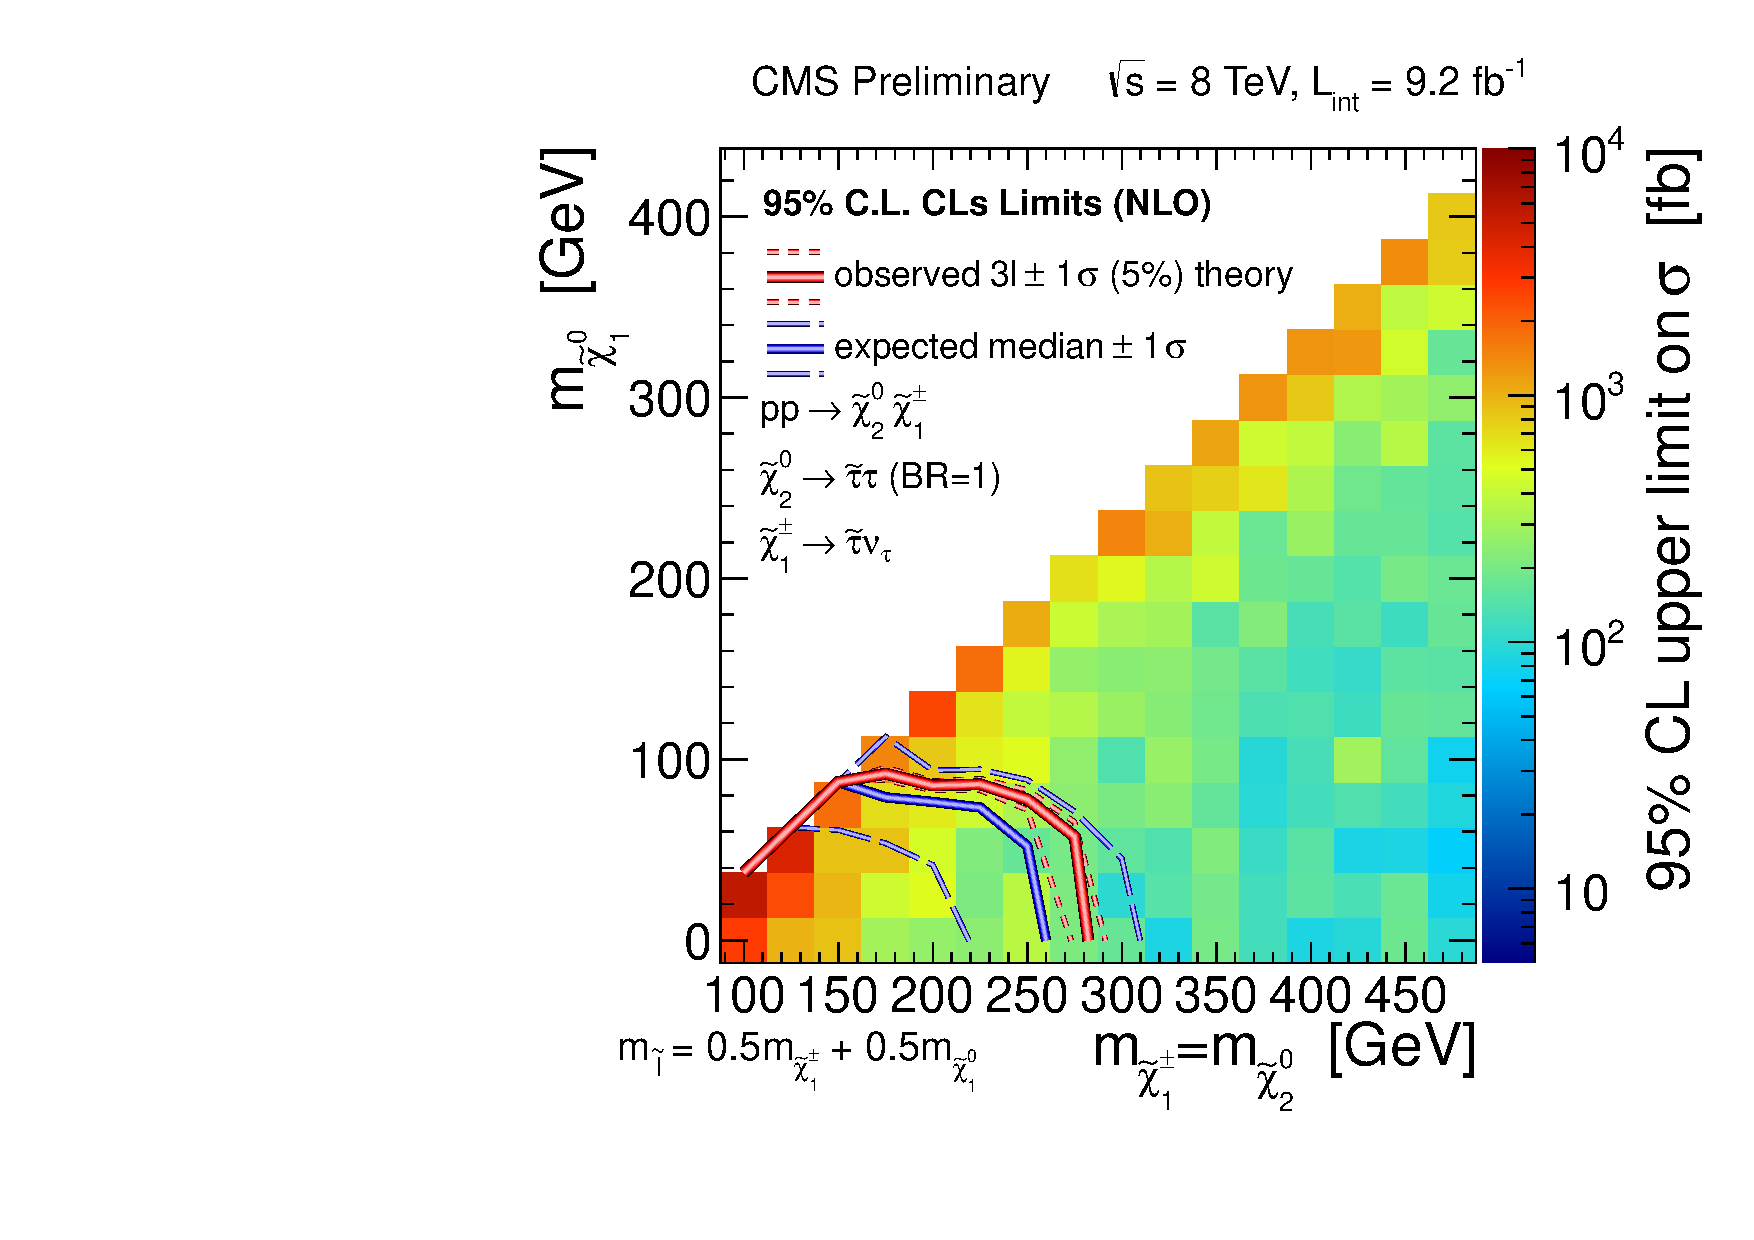
\includegraphics[width=0.8\textwidth]{plots/exclusions/exclusion_TChiStauSnu_0_5.pdf} }
%\subfigure[$\xslep = 0.95$]{\label{fig:ULtriC3}\includegraphics[width=0.33\textwidth]{plots/exclusions/xxx.pdf} }
\caption{The exclusion contours for $\tau$-dominated scenario corresponding to results in Figure~\ref{fig:ULtriA}. 
%(a) and (c) combination of 3-lepton searches with SS d-lepton analysis, 
%(b) 
%3 lepton searches.}
}
\label{fig:ULtriC}
\end{center}
\end{figure}
%==========================================================================================


%%%%%%%%%%%%%%%%%%%%%%%%%%%%%%%%%%%%%%%%%%%%%%%%
%%%%%%%%%%%%%%%%%%%%%%%%%%%%%%%%%%%%%%%%%%%%%%%%
\subsection{Limits on SMS with on-shell W and Z from WZ + $\ETmiss$ and three-lepton analyses}
For limits on the SMS with on-shell W and Z bosons, we 
show the results of the \wzmet analysis~\cite{AN-2012:254}, the three-lepton analysis as well as the combined result.
%From the \wzzmet analysis, we use the results in exclusive
%\MET regions, as summarized in Table~\ref{tab:results_targ}.  
%For the
%three-lepton analysis, we use the results shown in Fig~\ref{fig:OSSFMET}.

In the combination, the common signal-related systematic uncertainties
for luminosity, jet energy scale, lepton identification, trigger efficiency, and
misidentification of light-flavor jets as \bjetsnohyphen are 
considered to be 100\% correlated. For backgrounds, the only common systematic uncertainty
is that for the $\W\Z$ simulation, which is treated as 100\% correlated.  No
events in the data pass both signal selections.  For the backgrounds,
the overlap in the control sample is less than 1\%.  Thus the two
selections are treated as independent.

Figure~\ref{fig:WZetmiss} displays the observed limits for the
two individual analyses and the combination.  
%For large $\mchi$, the
%has higher sensitivity due to the large hadronic
%branching fractions of the $\W$ and $\Z$ bosons. At lower $\mchi$, the
%signal events do not have large $\MET$, resulting in a loss of signal
%region acceptance for the \wzzmet analysis. In this region, the
%background suppression provided by the requirement of a third lepton
%leads to better sensitivity for the three-lepton analysis.

%==========================================================================================
\begin{figure}[htp]
\begin{center}
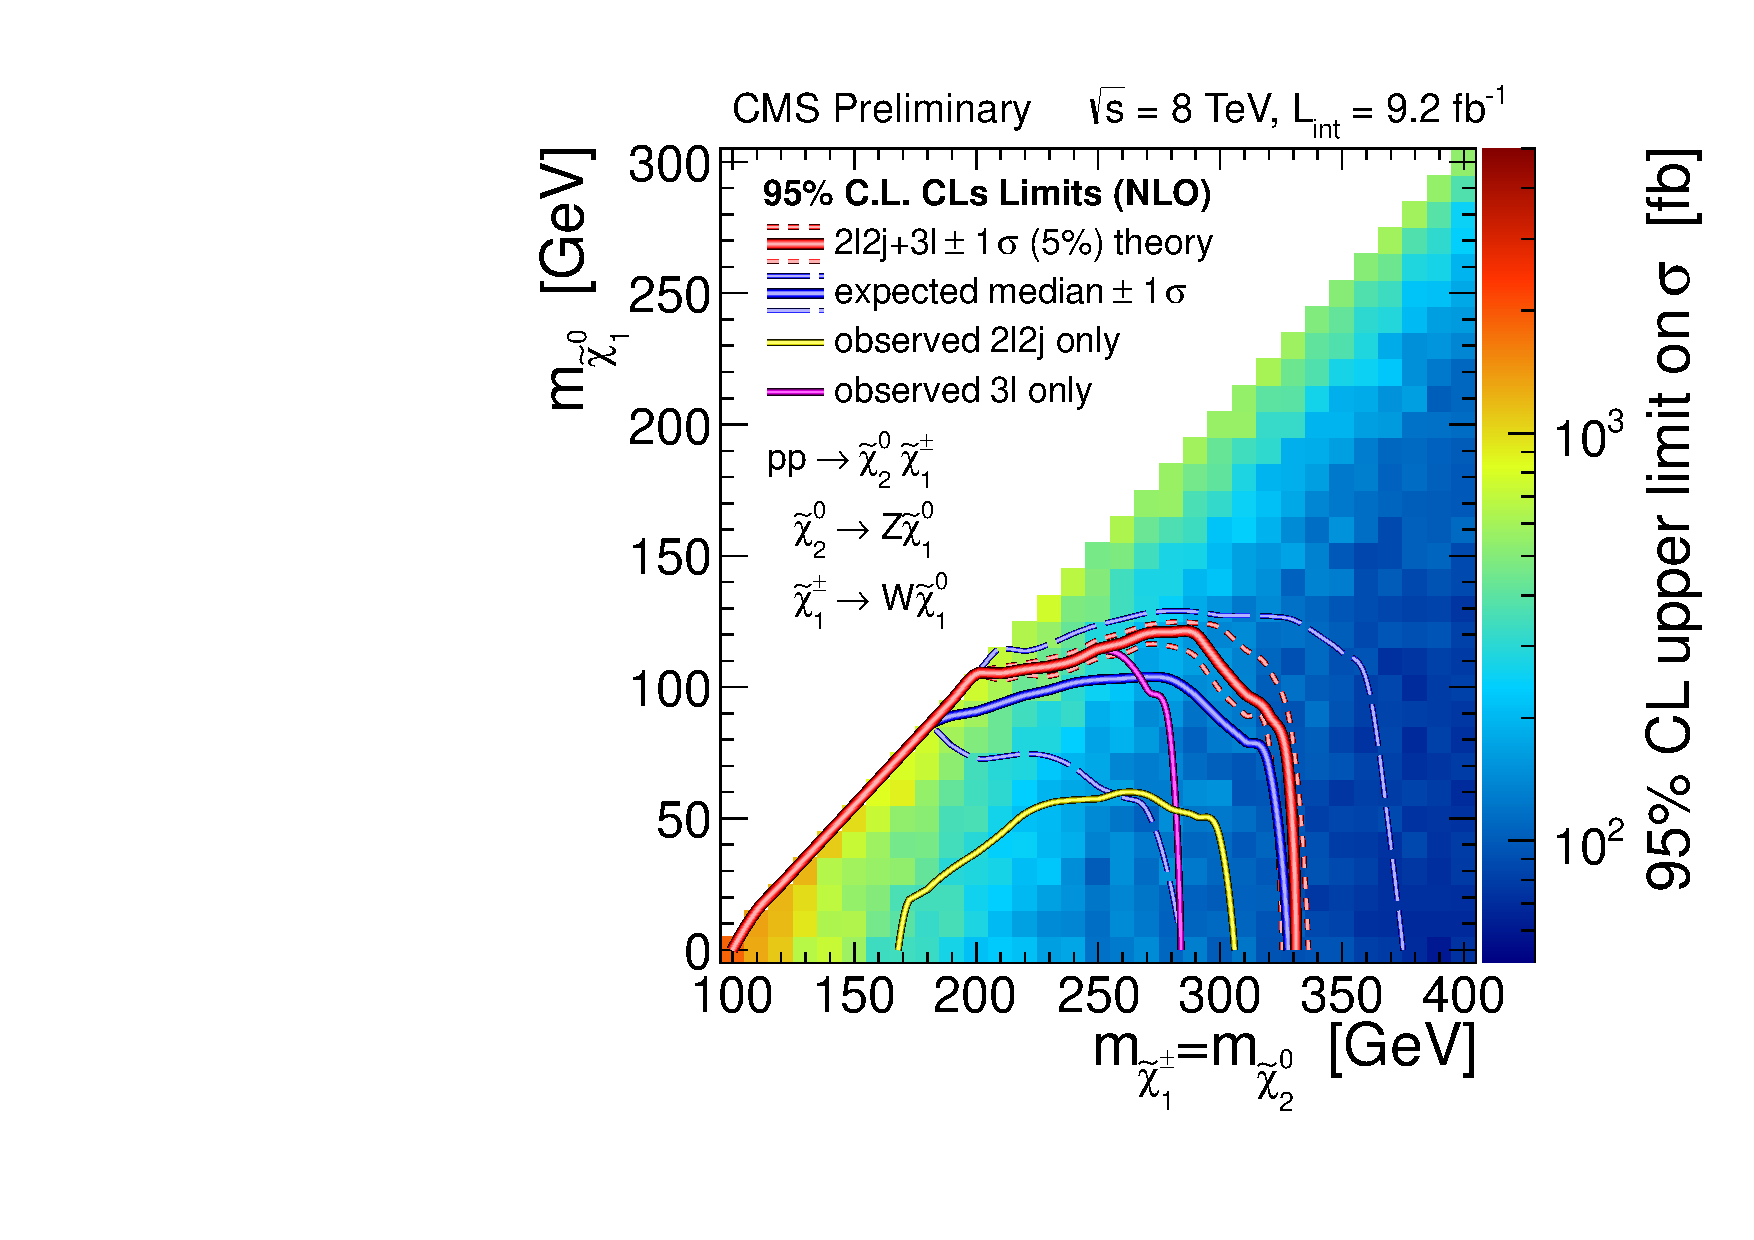
\includegraphics[width=0.8\textwidth]{plots/exclusions/exclusion_TChiWZ.pdf}
\caption{Interpretation of the WZ + $\ETmiss$ and three-lepton results in the context of the WZ 
SMS. The WZ+ $\ETmiss$ observed, three-lepton observed, combined observed, and combined
expected contours are indicated.}
\label{fig:WZetmiss}
\end{center}
\end{figure}
%==========================================================================================




